\documentclass{standalone}
\usepackage{tikz}
\usepackage{adjustbox}
\usepackage{helvet}  
\usepackage{sansmathfonts}  
\renewcommand{\familydefault}{\sfdefault}  
\usetikzlibrary{arrows.meta,calc,decorations.pathmorphing}
\usetikzlibrary{shapes.geometric, shapes.arrows}
\usepackage{xcolor}

\definecolor{colorFFFFFF}{HTML}{FFFFFF}
\definecolor{color000000}{HTML}{000000}
\definecolor{color001122}{HTML}{001122}
\begin{document}
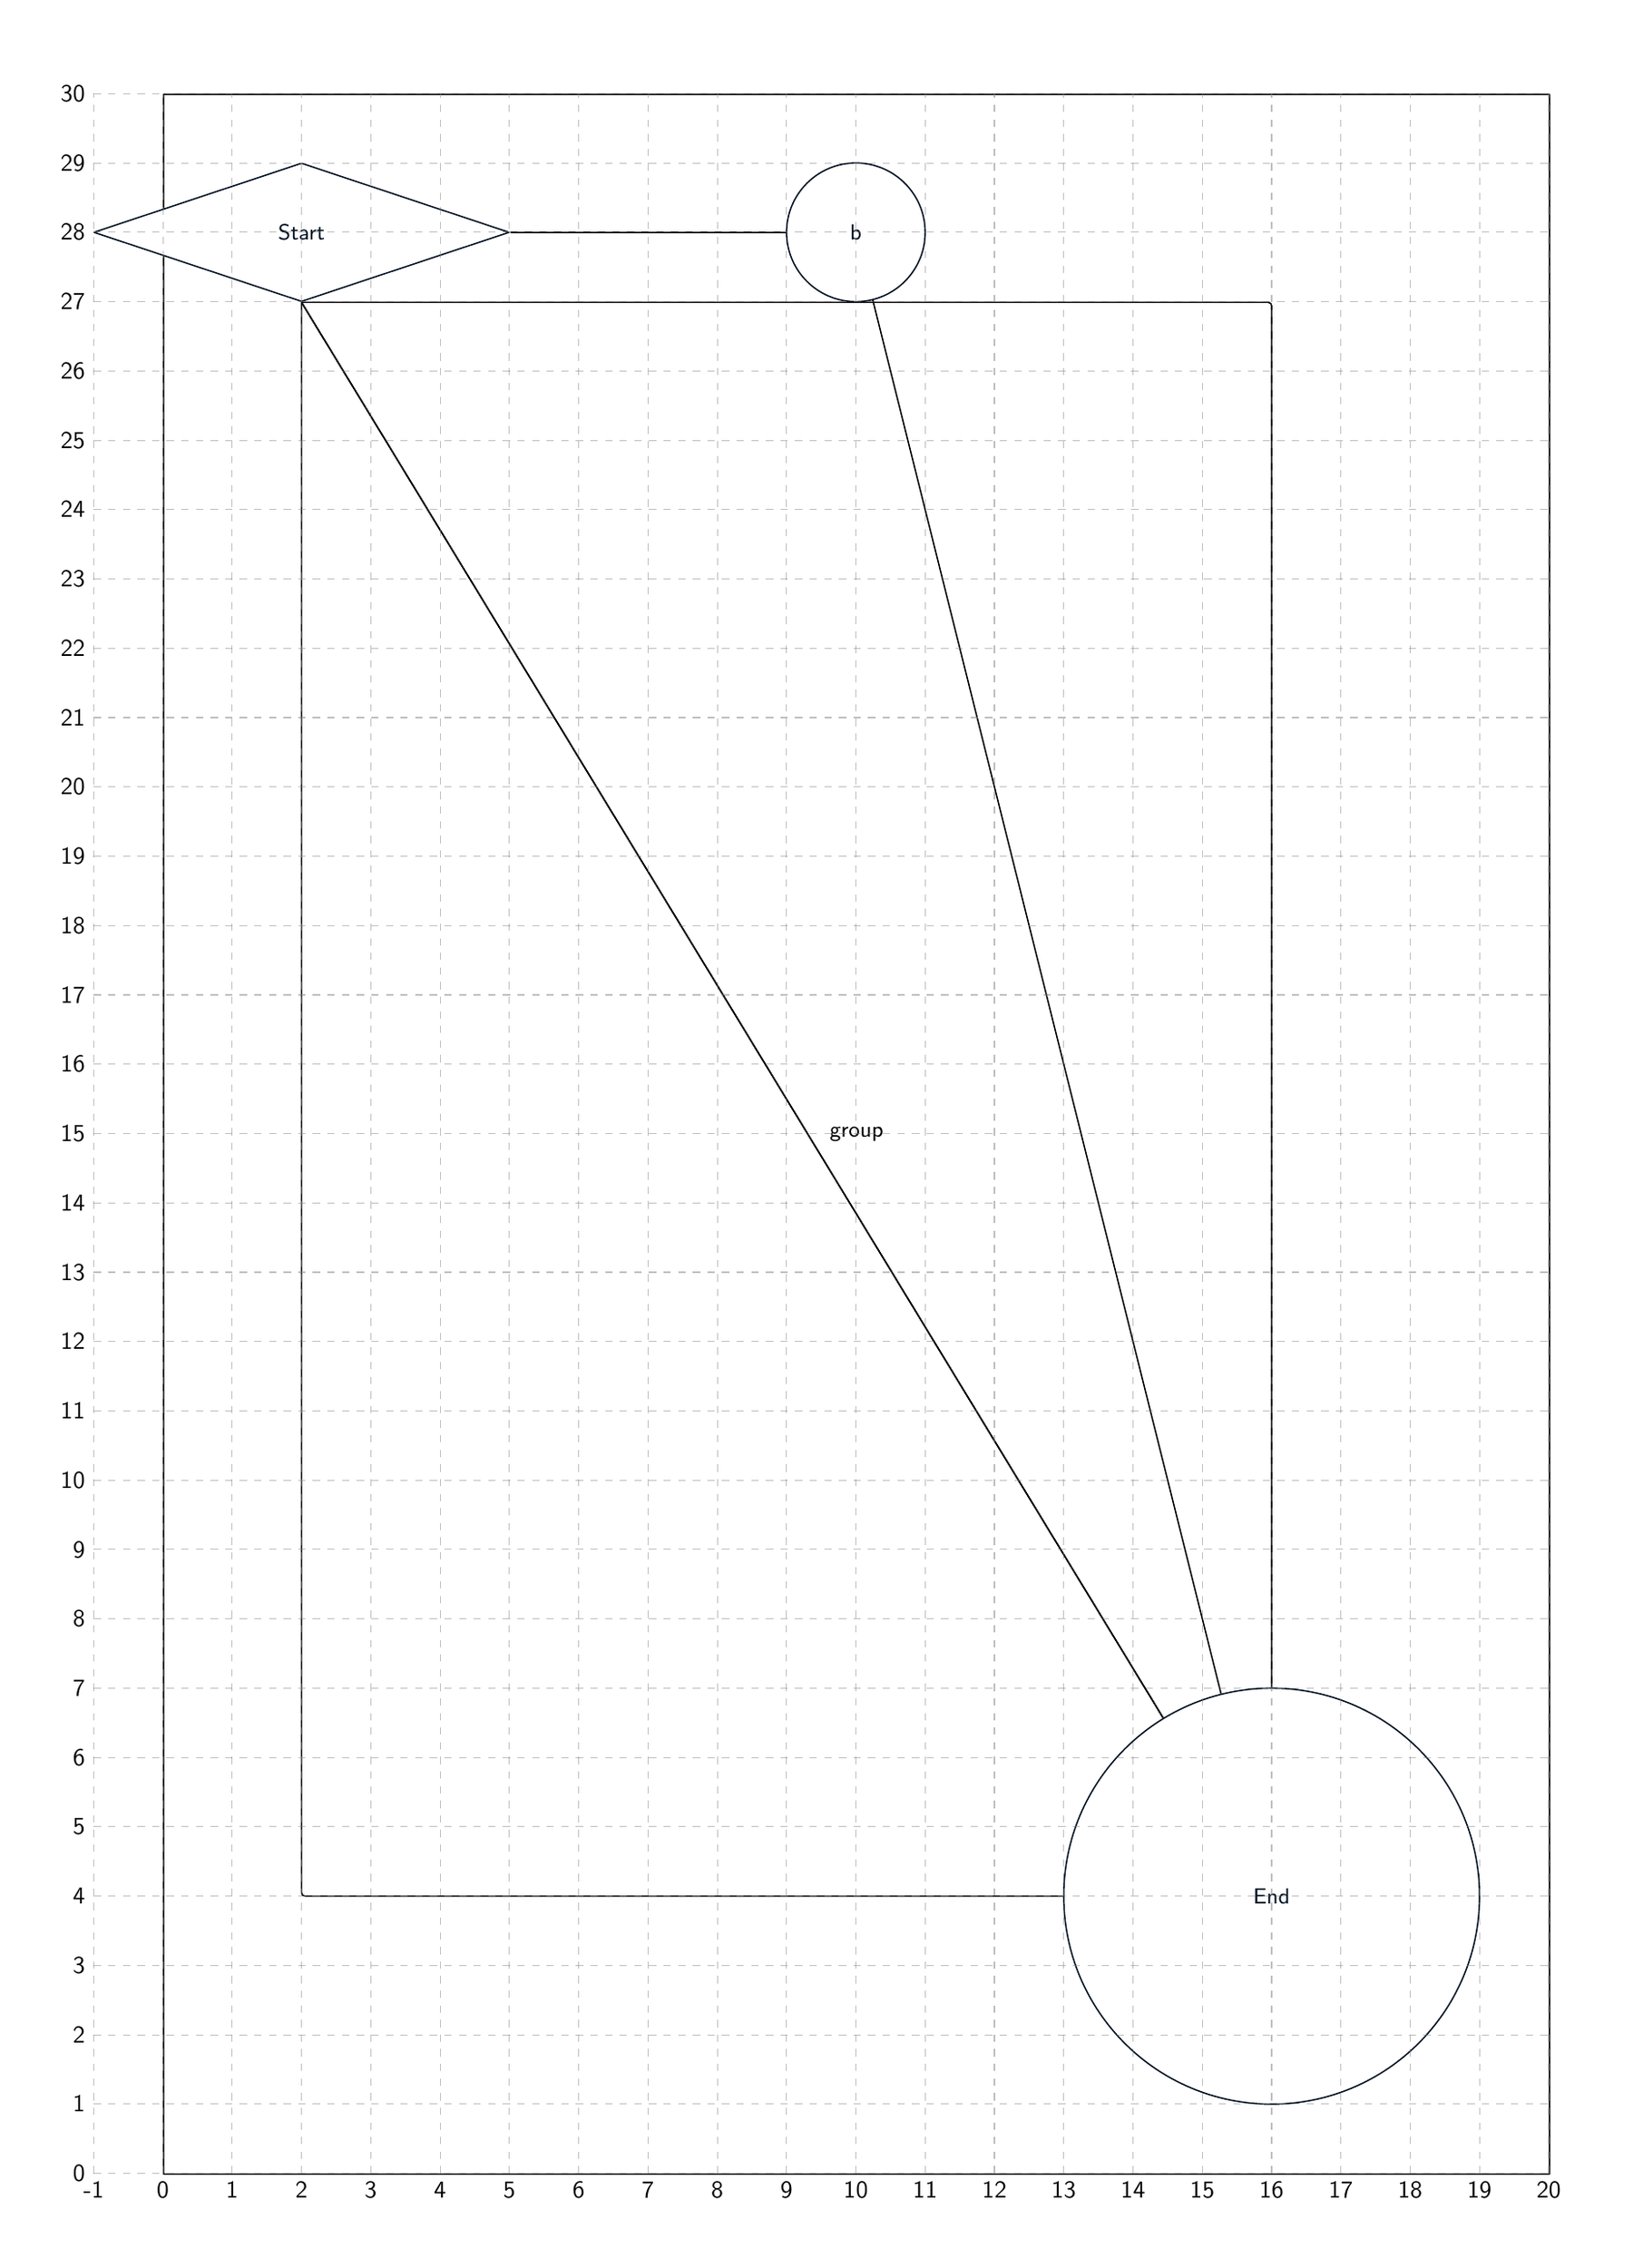
\begin{tikzpicture}
\useasboundingbox (-2,-1) rectangle (21,31);



\node[shape=rectangle, fill=colorFFFFFF, draw=color000000, minimum width=20cm, minimum height=30cm, rounded corners=0.005cm, line width=0.02cm, text opacity=1, font=\footnotesize, inner sep=0pt, anchor=north west] (group) at (0,30) {\adjustbox{max width=20cm, max height=30cm}{\small{\sffamily{group}}}};
\node[shape=diamond, fill=colorFFFFFF, draw=color001122, minimum width=6cm, minimum height=2cm, rounded corners=0.005cm, line width=0.02cm, text opacity=1, font=\footnotesize, inner sep=0pt, text=color001122] (start) at (2,28) {\adjustbox{max width=6cm, max height=2cm}{\textcolor{color001122}{\small{\sffamily{Start}}}}};
\node[shape=circle, fill=colorFFFFFF, draw=color001122, minimum width=6cm, minimum height=6cm, rounded corners=0.005cm, line width=0.02cm, text opacity=1, font=\footnotesize, inner sep=0pt, text=color001122] (end) at (16,4) {\adjustbox{max width=6cm, max height=6cm}{\textcolor{color001122}{\small{\sffamily{End}}}}};
\node[shape=circle, fill=colorFFFFFF, draw=color001122, minimum width=2cm, minimum height=2cm, rounded corners=0.005cm, line width=0.02cm, text opacity=1, font=\footnotesize, inner sep=0pt, text=color001122] (b) at (10,28) {\adjustbox{max width=2cm, max height=2cm}{\textcolor{color001122}{\small{\sffamily{b}}}}};
\draw[draw=color000000, line width=0.02cm, rounded corners=0.05cm] (start) to (b);
\draw[draw=color000000, line width=0.02cm, rounded corners=0.05cm] (b) to (end);
\draw[draw=color000000, line width=0.02cm, rounded corners=0.05cm] (start.south) to (end);
\draw[draw=color000000, line width=0.02cm, rounded corners=0.05cm] (start.south) -- (end);
\draw[draw=color000000, line width=0.02cm, rounded corners=0.05cm] (start.south) |- (end);
\draw[draw=color000000, line width=0.02cm, rounded corners=0.05cm] (start.south) -| (end);
\draw[dashed,gray,opacity=0.5] (-1,0) -- (-1,30);
\node[below] at (-1,0) {-1};
\draw[dashed,gray,opacity=0.5] (0,0) -- (0,30);
\node[below] at (0,0) {0};
\draw[dashed,gray,opacity=0.5] (1,0) -- (1,30);
\node[below] at (1,0) {1};
\draw[dashed,gray,opacity=0.5] (2,0) -- (2,30);
\node[below] at (2,0) {2};
\draw[dashed,gray,opacity=0.5] (3,0) -- (3,30);
\node[below] at (3,0) {3};
\draw[dashed,gray,opacity=0.5] (4,0) -- (4,30);
\node[below] at (4,0) {4};
\draw[dashed,gray,opacity=0.5] (5,0) -- (5,30);
\node[below] at (5,0) {5};
\draw[dashed,gray,opacity=0.5] (6,0) -- (6,30);
\node[below] at (6,0) {6};
\draw[dashed,gray,opacity=0.5] (7,0) -- (7,30);
\node[below] at (7,0) {7};
\draw[dashed,gray,opacity=0.5] (8,0) -- (8,30);
\node[below] at (8,0) {8};
\draw[dashed,gray,opacity=0.5] (9,0) -- (9,30);
\node[below] at (9,0) {9};
\draw[dashed,gray,opacity=0.5] (10,0) -- (10,30);
\node[below] at (10,0) {10};
\draw[dashed,gray,opacity=0.5] (11,0) -- (11,30);
\node[below] at (11,0) {11};
\draw[dashed,gray,opacity=0.5] (12,0) -- (12,30);
\node[below] at (12,0) {12};
\draw[dashed,gray,opacity=0.5] (13,0) -- (13,30);
\node[below] at (13,0) {13};
\draw[dashed,gray,opacity=0.5] (14,0) -- (14,30);
\node[below] at (14,0) {14};
\draw[dashed,gray,opacity=0.5] (15,0) -- (15,30);
\node[below] at (15,0) {15};
\draw[dashed,gray,opacity=0.5] (16,0) -- (16,30);
\node[below] at (16,0) {16};
\draw[dashed,gray,opacity=0.5] (17,0) -- (17,30);
\node[below] at (17,0) {17};
\draw[dashed,gray,opacity=0.5] (18,0) -- (18,30);
\node[below] at (18,0) {18};
\draw[dashed,gray,opacity=0.5] (19,0) -- (19,30);
\node[below] at (19,0) {19};
\draw[dashed,gray,opacity=0.5] (20,0) -- (20,30);
\node[below] at (20,0) {20};
\draw[dashed,gray,opacity=0.5] (-1,0) -- (20,0);
\node[left] at (-1,0) {0};
\draw[dashed,gray,opacity=0.5] (-1,1) -- (20,1);
\node[left] at (-1,1) {1};
\draw[dashed,gray,opacity=0.5] (-1,2) -- (20,2);
\node[left] at (-1,2) {2};
\draw[dashed,gray,opacity=0.5] (-1,3) -- (20,3);
\node[left] at (-1,3) {3};
\draw[dashed,gray,opacity=0.5] (-1,4) -- (20,4);
\node[left] at (-1,4) {4};
\draw[dashed,gray,opacity=0.5] (-1,5) -- (20,5);
\node[left] at (-1,5) {5};
\draw[dashed,gray,opacity=0.5] (-1,6) -- (20,6);
\node[left] at (-1,6) {6};
\draw[dashed,gray,opacity=0.5] (-1,7) -- (20,7);
\node[left] at (-1,7) {7};
\draw[dashed,gray,opacity=0.5] (-1,8) -- (20,8);
\node[left] at (-1,8) {8};
\draw[dashed,gray,opacity=0.5] (-1,9) -- (20,9);
\node[left] at (-1,9) {9};
\draw[dashed,gray,opacity=0.5] (-1,10) -- (20,10);
\node[left] at (-1,10) {10};
\draw[dashed,gray,opacity=0.5] (-1,11) -- (20,11);
\node[left] at (-1,11) {11};
\draw[dashed,gray,opacity=0.5] (-1,12) -- (20,12);
\node[left] at (-1,12) {12};
\draw[dashed,gray,opacity=0.5] (-1,13) -- (20,13);
\node[left] at (-1,13) {13};
\draw[dashed,gray,opacity=0.5] (-1,14) -- (20,14);
\node[left] at (-1,14) {14};
\draw[dashed,gray,opacity=0.5] (-1,15) -- (20,15);
\node[left] at (-1,15) {15};
\draw[dashed,gray,opacity=0.5] (-1,16) -- (20,16);
\node[left] at (-1,16) {16};
\draw[dashed,gray,opacity=0.5] (-1,17) -- (20,17);
\node[left] at (-1,17) {17};
\draw[dashed,gray,opacity=0.5] (-1,18) -- (20,18);
\node[left] at (-1,18) {18};
\draw[dashed,gray,opacity=0.5] (-1,19) -- (20,19);
\node[left] at (-1,19) {19};
\draw[dashed,gray,opacity=0.5] (-1,20) -- (20,20);
\node[left] at (-1,20) {20};
\draw[dashed,gray,opacity=0.5] (-1,21) -- (20,21);
\node[left] at (-1,21) {21};
\draw[dashed,gray,opacity=0.5] (-1,22) -- (20,22);
\node[left] at (-1,22) {22};
\draw[dashed,gray,opacity=0.5] (-1,23) -- (20,23);
\node[left] at (-1,23) {23};
\draw[dashed,gray,opacity=0.5] (-1,24) -- (20,24);
\node[left] at (-1,24) {24};
\draw[dashed,gray,opacity=0.5] (-1,25) -- (20,25);
\node[left] at (-1,25) {25};
\draw[dashed,gray,opacity=0.5] (-1,26) -- (20,26);
\node[left] at (-1,26) {26};
\draw[dashed,gray,opacity=0.5] (-1,27) -- (20,27);
\node[left] at (-1,27) {27};
\draw[dashed,gray,opacity=0.5] (-1,28) -- (20,28);
\node[left] at (-1,28) {28};
\draw[dashed,gray,opacity=0.5] (-1,29) -- (20,29);
\node[left] at (-1,29) {29};
\draw[dashed,gray,opacity=0.5] (-1,30) -- (20,30);
\node[left] at (-1,30) {30};

\end{tikzpicture}
\end{document}